\chapter{Accuracy and Bandwidth Verification} \label{App:AccuracyBWTest}
This appendix documents the test setups and test results for requirements §3, §4, §5 from the requirements in table \refq{tab:5_SystemRequirements} in chapter\refq{ch:SystemRequirements}.

\subsection{§3 Impedance Range Verification} \label{subsec:ZRangeVerify} 
The requirements states that instrument should be able to measure an impedance in the interval $10m\Omega < |Z| < 100M \Omega$. To test this requirement, the instrument is tested in both extremes of this range. An impedance reference, or precision calibrator, is not available for the project to use so a \SIQ{100}{\mega\ohm} resistor and a \SIQ{10}{\milli\ohm} resistor was made by placing multiple resistors in series/parallel.

\subsubsubsection{Verify \SIQ{100}{\mega\ohm} resistor and \SIQ{10}{\milli\ohm} resistor}

The \SIQ{100}{\mega\ohm} resistor is a series connection of 10 \SIQ{10}{\mega\ohm} resistors. The actual resistance must be known before testing the instrument. No available multimeter, or other instrument, was available to measure this, instead several DC power supplies are placed in series to supply \SIQ{320}{\volt}DC and the current through the resistor is measured with a 34401A DMM while the voltage across it is measured with another 34401 as seen on figure \refq{fig:App_A_Z_100MEGSetup}.

\begin{figure}[H]
    \centering
    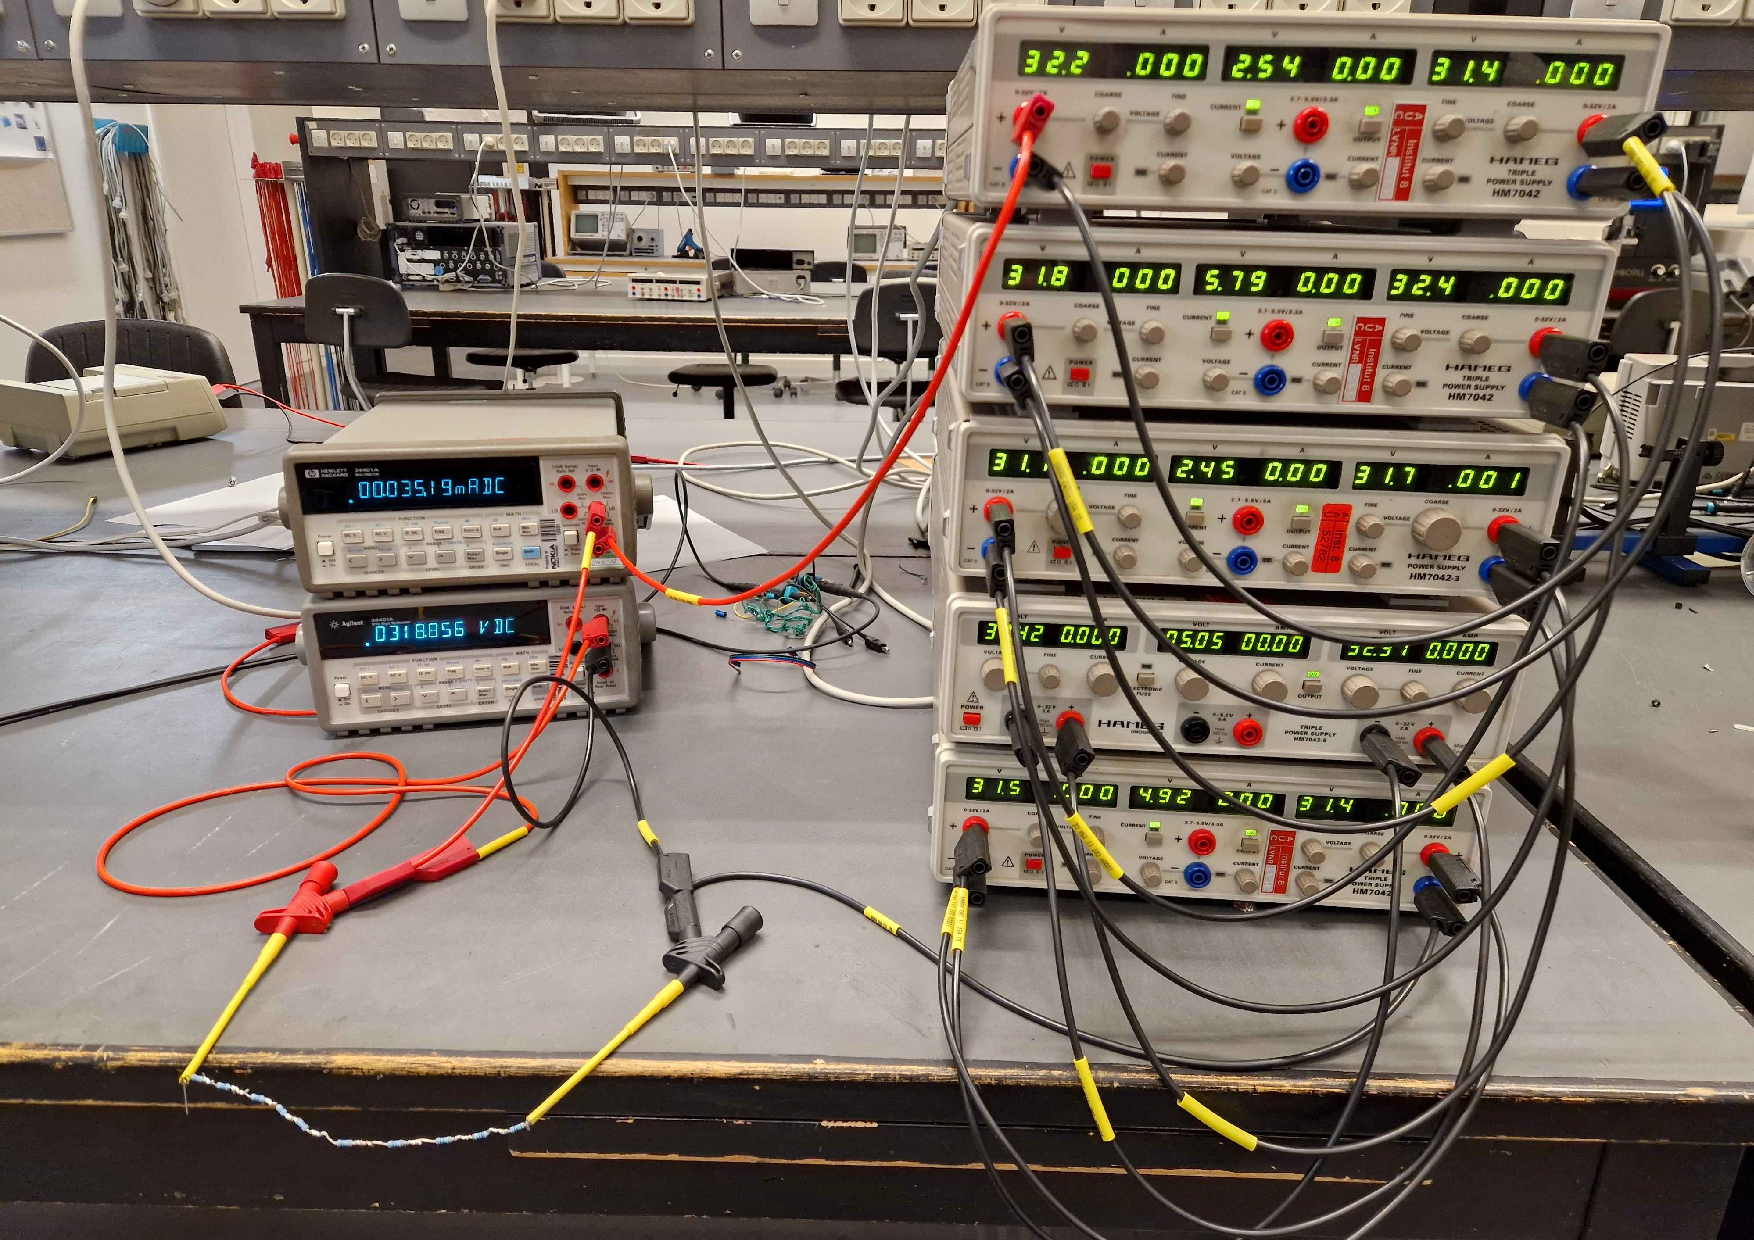
\includegraphics[clip, trim=0 0 0 0, width=0.75\textwidth]{Appendix/Figures/A_Z_100MegSetup.pdf}
    \caption{Several DC power supplies is set in series to produce 320VDC. The current through the resistor and the voltage across it is measured with two DMMs.}
    \label{fig:App_A_Z_100MEGSetup}
\end{figure}

The voltage across the resistor is $V_R = \SIQ{318.86}{\volt}$ while the current through it is $I_R = \SIQ{35.19}{\micro\ampere}$. The input impedance of the current measuring DMM is neglible while the voltage measuring DMM has an input impedance of \SIQ{10}{\mega\ohm}. The resistance is $R_{100M} = \SIQ{96.5}{\mega\ohm}$ as shown in eq \refq{eq:A_Z_100MegTest}.

\begin{equation}\label{eq:A_Z_100MegTest}
    \begin{split}
        \frac{V_R}{I_R} = ((Z_{INDMM})^{-1} + (R_{100M})^{-1})^{-1}\\
        R_{100M} = \frac{V_R Z_{INDMM}}{I_R Z_{INDMM}-V_R}\\
        R_{100M} = \frac{318.86 \cdot 10E6}{(35.18E-6)(10E6) + 318.86} = 9.6507E7
    \end{split}
\end{equation}

THe \SIQ{10}{\milli\ohm} resistor is a parallel connection of 10 \SIQ{100}{\milli\ohm} resistors. This resistor was also verified by letting a DC current pass through it and measuring the voltage across it. The test setup can be seen on figure \refq{fig:App_A_Z_100MilliSetup}.

\begin{figure}[H]
    \centering
    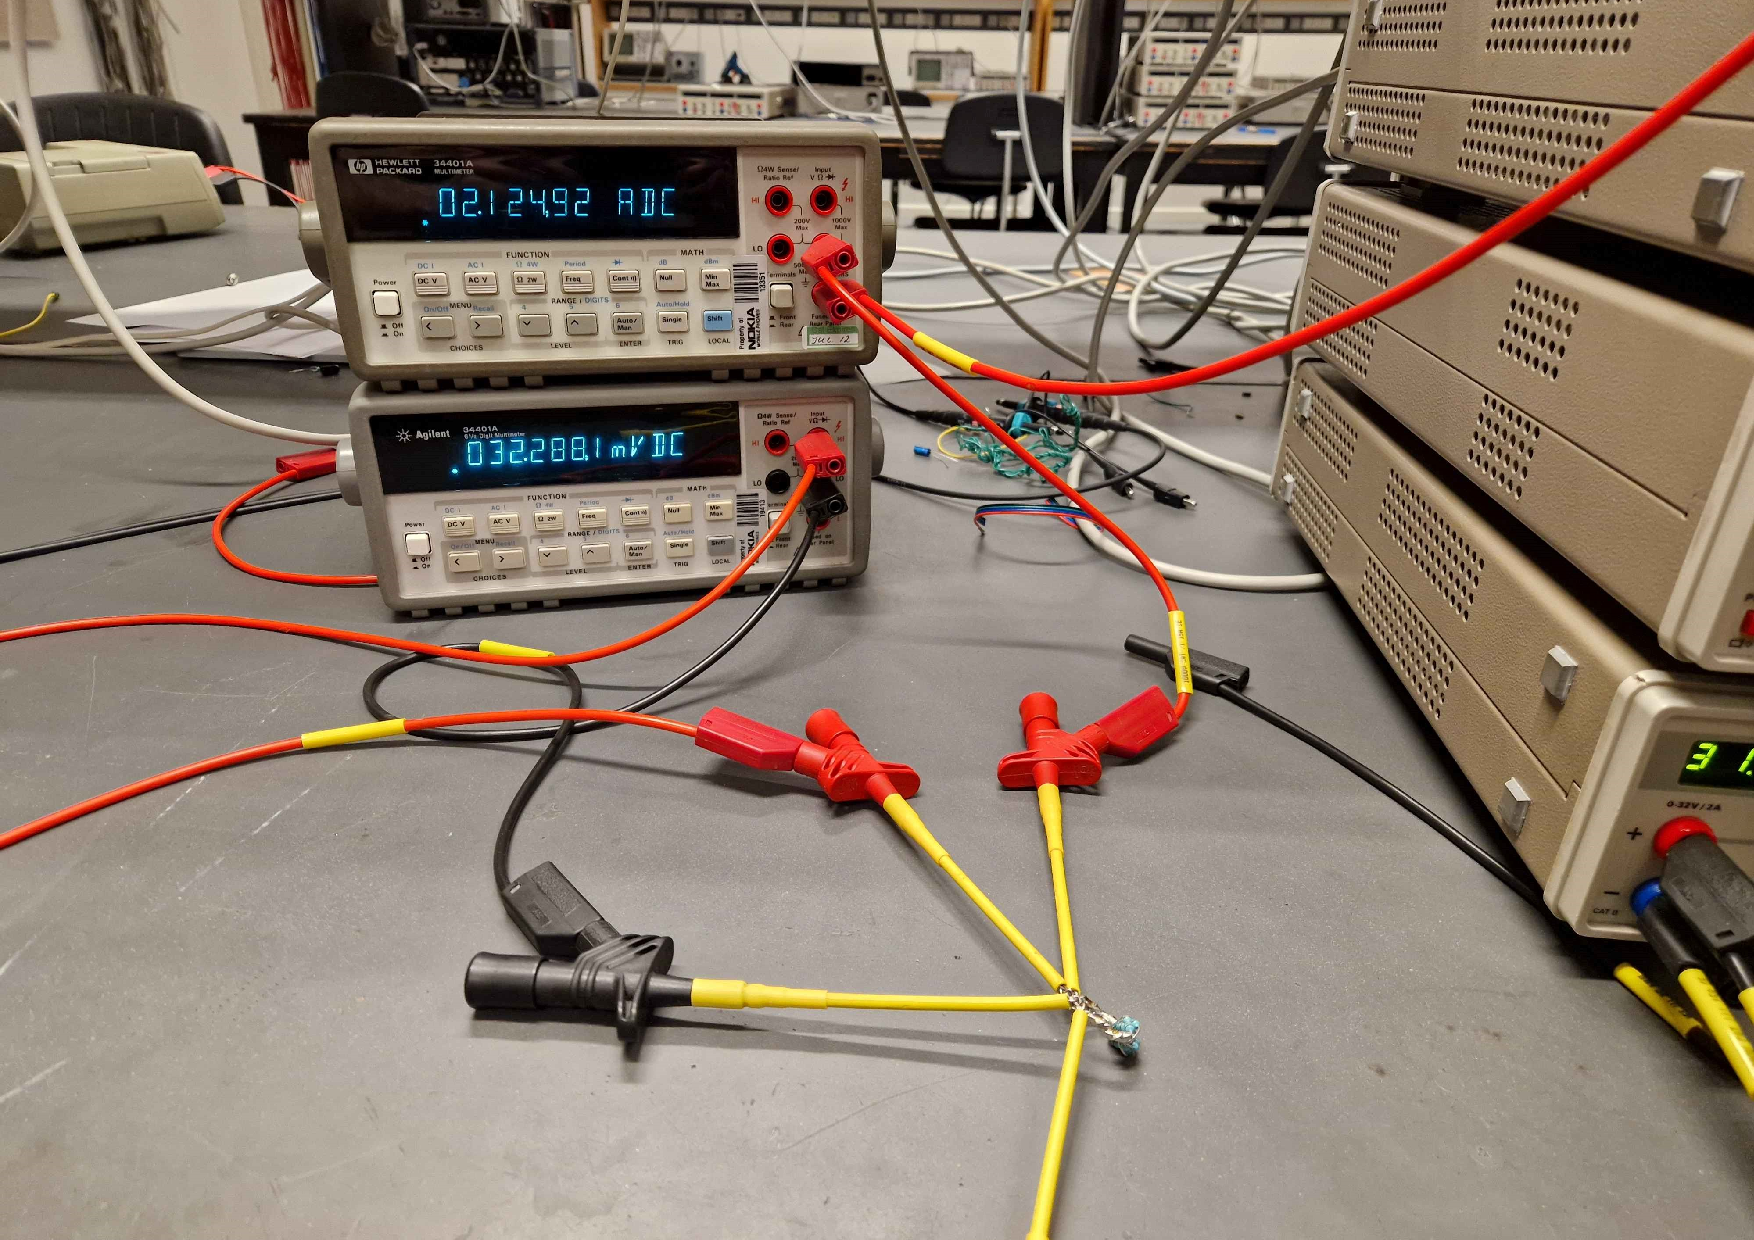
\includegraphics[clip, trim=0 0 0 0, width=0.75\textwidth]{Appendix/Figures/A_Z_10MilliSetup.pdf}
    \caption{A DC power supply is connected to the \SIQ{10}{\milli\ohm} resistor and the current through and voltage across it is measured with two DMMS.}
    \label{fig:App_A_Z_100MilliSetup}
\end{figure}

The voltage across the resistor is $V_{10MIL} = \SIQ{32.2881}{\milli\volt}$ the current through it is $I_{10MIL} = \SIQ{2.12492}{\ampere}$ so the resistor has a value of $R_{10MIL} =\SIQ{15.195}{\milli\ohm}$.

\subsubsubsection{Test results}

The $R_{100MEG} = \SIQ{96.5}{\mega\ohm}$ and $R_{10MIL} =\SIQ{15.195}{\milli\ohm}$ resistors have been measured by the instrument and the results can be seen in table \refq{tab:A_Z_ZRANGE_RESULT_TAB}. 

\begin{table}[H]
    \centering
    \renewcommand{\arraystretch}{1.5}
    \setlength{\tabcolsep}{8pt}
    \begin{tabular}{|c|c|c|c|c|c|}
    \hline
    \textbf{Resistor} & \textbf{Nom. Value} & \textbf{Meas. Value} & \textbf{Deviation} & \textbf{Requirement} & \textbf{Verdict} \\ \hline
    $R_{10MIL}$ & \SIQ{15.195}{\milli\ohm} & \SIQ{14.978}{\milli\ohm} & 1.428\% & $\pm$ 2\% & Pass  \\ \hline
    $R_{100MEG}$ & \SIQ{96.5}{\mega\ohm} & \SIQ{98.63}{\mega\ohm} & -2.207\% & $\pm$2\% & Fail \\ \hline
    \end{tabular}
    \caption{Test results for the measurements. The Nom. Value is the confirmed values of the test resistors. The Measured Value is the reading from the impedance analyzer. }
    \label{tab:A_Z_ZRANGE_RESULT_TAB}
    \end{table}

    The \SIQ{10}{\milli\ohm} range is passed, while the \SIQ{100}{\mega\ohm} range is failed as per for the requirement.  

    \subsection{§4, §5 Modulus and Phase Accuracy Verification} \label{subsec:ModulusAccuracyTest} 

    The accuracy of the impedance has been measured at various test frequencies. The DUTs for this test will be \SIQ{10}{\ohm}, \SIQ{10}{\kilo\ohm} and \SIQ{100}{\kilo\ohm}. Capacitors were also tested, their values are \SIQ{27}{\pico\farad},\SIQ{150}{\nano\farad} and \SIQ{1}{\micro\farad}. An inductor was also tested it has the value \SIQ{100}{\micro\henry}.
    
    The results for the resistors can be seen in table \refq{tab:A_Z_ImpedanceMeasurementWIthResistor}. The resistors are assumed to be ideal, so the phase is assumed to be $0\degree$ any deviation from this is an error.

        \begin{table}[H]
            \centering
            \renewcommand{\arraystretch}{1.5}
            \setlength{\tabcolsep}{8pt}
            \begin{tabular}{|c|c|c|c|c|c|c|}
            \hline
            \textbf{Resistor} & \textbf{Tol.} & \textbf{Meas. Z Value} & \textbf{Act. Res.} & \textbf{Dev. M} & \textbf{Dev. Arg} & \textbf{Freq} \\ \hline
            \SIQ{10}{\ohm} & 0.1\% & $9.9972 \angle -0.0091\degree$ & 9.9972 & 0.0256\% & $-0.0091\degree$ & \SIQ{1}{\kilo\hertz} \\ \hline
            \SIQ{10}{\ohm} & 0.1\% & $1.0000E1 \angle -0.4845\degree$ & 1.0000E1 & 0\% & $-0.4845\degree$ & \SIQ{50}{\kilo\hertz} \\ \hline
            \SIQ{10}{\ohm} & 0.1\% & $9.9995 \angle -2.5329\degree$ & 9.9995 & 0.005\% & $-2.5329\degree$ & \SIQ{250}{\kilo\hertz} \\ \hline
            \SIQ{10}{\kilo\ohm} & 0.1\% & $9.9974E3 \angle 0.0008\degree$ & 9.9974E3 & 0.026\% & $0.0008\degree$ & \SIQ{1}{\kilo\hertz} \\ \hline
            \SIQ{10}{\kilo\ohm} & 0.1\% & $9.9998E3 \angle -0.2289\degree$ & 9.9998E3 & 0.002\% & $-0.2289\degree$ & \SIQ{50}{\kilo\hertz} \\ \hline
            \SIQ{10}{\kilo\ohm} & 0.1\% & $9.9996E3 \angle -3.1832\degree$ & 9.9996E3 & 0.004\% & $-3.1832\degree$ & \SIQ{250}{\kilo\hertz} \\ \hline
            \SIQ{100}{\kilo\ohm} & 0.1\% & $1.0002E5 \angle -0.0045\degree$ & 1.0002E5 & -0.02\% & $-0.0045\degree$ & \SIQ{1}{\kilo\hertz} \\ \hline
            \SIQ{100}{\kilo\ohm} & 0.1\% & $9.9860E4 \angle -0.6684\degree$ & 9.9860E4 & 0.14\% & $-0.6684\degree$ & \SIQ{50}{\kilo\hertz} \\ \hline
            \SIQ{100}{\kilo\ohm} & 0.1\% & $1.0159E5 \angle -3.0477\degree$ & 1.0159E5 & -1.59\% & $-3.0477\degree$ & \SIQ{250}{\kilo\hertz} \\ \hline
            \end{tabular}
            \caption{Resistor Measurements at various test frequencies. The tolerance is the tolerance that the manufacturer has listed for the component.}
            \label{tab:A_Z_ImpedanceMeasurementWIthResistor}
        \end{table}
        

        The results for the Capacitors can be seen in table \refq{tab:A_Z_ImpedanceMeasurementWIthCapacitor}. It is assumed that the ESR of the capacitors is zero. The impedance that is used for calculating the deviation will simply be the capacitive reactance of each capacitor, $X_C = 1/(\omega C)$. The ideal angle of the impedance is assumed to be $-90\degree$. 
        
            \begin{table}[H]
                \centering
                \renewcommand{\arraystretch}{1.5}
                \setlength{\tabcolsep}{8pt}
                \begin{tabular}{|c|c|c|c|c|c|c|}
                \hline
                \textbf{Capacitor} & \textbf{Tol.} & \textbf{Meas. Z Value} & \textbf{Dev. M} & \textbf{Dev. Arg} & \textbf{Freq.} \\ \hline
                \SIQ{27}{\pico\farad} & 2\% & $5.8441E6 \angle -89.9512\degree$ & -0.865\% & $-0.0488\degree$ & \SIQ{1}{\kilo\hertz} \\ \hline
                \SIQ{27}{\pico\farad} & 2\% & $1.1779E5 \angle -90.0712\degree$ & 0.0890\% & $0.0712\degree$ & \SIQ{50}{\kilo\hertz} \\ \hline
                \SIQ{27}{\pico\farad} & 2\% & $2.3447E4 \angle -91.2208\degree$ & 0.5578\% & $1.2208\degree$ & \SIQ{250}{\kilo\hertz} \\ \hline
                \SIQ{150}{\nano\farad} & 1\% & $1.0662E3 \angle -90.0170\degree$ & -0.4870\% & $0.017\degree$ & \SIQ{1}{\kilo\hertz} \\ \hline
                \SIQ{150}{\nano\farad} & 1\% & $2.1294E1 \angle -90.2847\degree$ & -0.3456\% & $0.2847\degree$ & \SIQ{50}{\kilo\hertz} \\ \hline
                \SIQ{150}{\nano\farad} & 1\% & $4.2473 \angle -92.0207\degree$ & -0.0746\% & $2.0207\degree$ & \SIQ{250}{\kilo\hertz} \\ \hline
                \SIQ{1}{\micro\farad} & 1\% & $1.5873E2 \angle -89.9869\degree$ & 0.2670\% & $-0.0131\degree$ & \SIQ{1}{\kilo\hertz} \\ \hline
                \SIQ{1}{\micro\farad} & 1\% & $3.1729 \angle -90.3050\degree$ & 0.3204\% & $0.3050\degree$ & \SIQ{50}{\kilo\hertz} \\ \hline
                \SIQ{1}{\micro\farad} & 1\% & $6.4378E-1 \angle -89.1977\degree$ & -1.1247\% & $-0.8023\degree$ & \SIQ{250}{\kilo\hertz} \\ \hline
                \end{tabular}
                \caption{Capacitor Measurements at various test frequencies. The tolerance is the tolerance that the manufacturer has listed for the component.}
                \label{tab:A_Z_ImpedanceMeasurementWIthCapacitor}
            \end{table}


            The results for the inductor can be seen in table \refq{tab:A_Z_ImpedanceMeasurementWIthInductor}. It is assumed that the ESR of the inductor is zero. The impedance that is used for calculating the deviation will simply be the inductive reactance of the inductor $X_L = \omega L$. The ideal angle of the impedance is assumed to be $90\degree$. 

                \begin{table}[H]
                    \centering
                    \renewcommand{\arraystretch}{1.5}
                    \setlength{\tabcolsep}{8pt}
                    \begin{tabular}{|c|c|c|c|c|c|}
                    \hline
                    \textbf{Inductor} & \textbf{Tol.} & \textbf{Meas. Value} & \textbf{Dev. M} & \textbf{Dev. Arg} & \textbf{Freq.} \\ \hline
                    \SIQ{100}{\micro\henry} & 5\% & $8.962E-1 \angle 43.3721\degree$ & $-42.6347\%$ & $46.6279\degree$ & \SIQ{1}{\kilo\hertz} \\ \hline
                    \SIQ{100}{\micro\henry} & 5\% & $3.0463E1 \angle 88.3468\degree$ & $3.0333 \%$ & $1.6532\degree$ & \SIQ{50}{\kilo\hertz} \\ \hline
                    \SIQ{100}{\micro\henry} & 5\% & $1.5095E2 \angle 88.178\degree$ & $3.9022 \%$ & $1.822\degree$ & \SIQ{250}{\kilo\hertz} \\ \hline
                    \end{tabular}
                    \caption{Inductor Measurements at various test frequencies. The tolerance is the tolerance that the manufacturer has listed for the component.}
                    \label{tab:A_Z_ImpedanceMeasurementWIthInductor}
                \end{table}

                The inductor measurement at $f_{test} = 1kHz$ will be disregarded as the ESR of the inductor is substantial and cannot be ignored at this frequency.